% Soubory musí být v kódování, které je nastaveno v příkazu \usepackage[...]{inputenc}

\documentclass[%
%  draft,       % Testovací překlad
  12pt,        % Velikost základního písma je 12 bodů
  a4paper,     % Formát papíru je A4
%  oneside,      			% Jednostranný tisk (výchozí)
%% Z následujicich voleb lze použít maximálně jednu:
%	dvipdfm  						% výstup bude zpracován programem 'dvipdfm' do PDF
%	dvips	  						% výstup bude zpracován programem 'dvips' do PS
%	pdftex							% překlad bude proveden programem 'pdftex' do PDF (výchozí)
%% Z následujících voleb lze použít jen jednu:
% english,            % originální jazyk je angličtina
% slovak,             % originální jazyk je slovenčina
czech              % originální jazyk je čeština (výchozí)
]{report}				    	% Dokument třídy 'zpráva'

\usepackage[utf8]		%	Kódování zdrojových souborů je Windows-1250
	{inputenc}					% Balíček pro nastavení kódování zdrojových souborů

\usepackage{graphicx} % Balíček 'graphicx' pro vkládání obrázků
											% Nutné pro vložení log školy a fakulty

\usepackage[
	nohyperlinks				% Nebudou tvořeny hypertextové odkazy do seznamu zkratek
]{acronym}						% Balíček 'acronym' pro sazby zkratek a symbolů
											% Nutné pro použití prostředí 'seznamzkratek' balíčku 'thesis'

\usepackage[
	unicode,						% Záložky a informace budou v kódování unicode
	breaklinks=true,		% Hypertextové odkazy mohou obsahovat zalomení řádku
	hypertexnames=false % Názvy hypertextových odkazů budou tvořeny
											% nezávisle na názvech TeXu
]{hyperref}						% Balíček 'hyperref' pro sazbu hypertextových odkazů
											% Nutné pro použití příkazu 'nastavenipdf' balíčku 'thesis'

\usepackage{pdfpages} % Balíček umožňující vkládat stránky z PDF souborů
                      % Nutné při vkládání titulních listů a zadání přímo
                      % ve formátu PDF z informačního systému

\usepackage{enumitem} % Balíček pro nastavení mezerování v odrážkách
  \setlist{topsep=0pt,partopsep=0pt,noitemsep}

\usepackage{cmap} 		% Balíček cmap zajišťuje, že PDF vytvořené `pdflatexem' je
											% plně "prohledávatelné" a "kopírovatelné"

\usepackage{upgreek}	% Balíček pro sazbu stojatých řeckých písmem
											% např. stojaté pí: \uppi
											% např. stojaté mí: \upmu (použitelné třeba v mikrometrech)
											% pozor, grafická nekompatibilita s fonty typu Computer Modern!

%% Nastavení českého jazyka při sazbě v češtině.
% Pro sazbu češtiny je možné použít mezinárodní balíček 'babel', jenž
% použití doporučujeme pro nové instalace (MikTeX2.8,TeXLive2009), nebo
% národní balíček 'czech', který doporučujeme ve starších instalacích.
% Balíček 'babel' bude správně fungovat pouze ve spojení s programy
% 'latex', 'pdflatex', zatímco balíček 'czech' bude fungovat ve spojení
% s programy 'cslatex', 'pdfcslatex'.
% Varianta A:
\usepackage    				
  {babel}             % Balíček pro sazbu různojazyčných dokumentů; kompilovat (pdf)latexem!
  										% převezme si z parametrů třídy správný jazyk
\usepackage{lmodern}	% vektorové fonty Latin Modern, nástupce půvoních Knuthových Computern Modern fontů
\usepackage{textcomp} % Dodatečné symboly
\usepackage[T1]{fontenc}  % Kódování fontu - mj. kvůli správným vzorům pro dělení slov
% Varianta B:
%\usepackage{czech}   % Alternativní balíček pro sazbu v českém jazyce, kompilovat (pdf)cslatexem!

\usepackage[%
%% Z následujících voleb lze použít pouze jednu
% left,               % Rovnice a popisky plovoucich objektů budou %zarovnány vlevo
  center,             % Rovnice a popisky plovoucich objektů budou zarovnány na střed (vychozi)
%% Z následujících voleb lze použít pouze jednu
%	phd
% treatise
% diploma							% sazba diplomové práce
% bachelor						%	sazba bakalářské práce
semestral						%	sazba zprávy semestrálního projektu
]{thesis}             % Balíček pro sazbu studentských prací
                      % Musí být vložen až jako poslední, aby
                      % ostatní balíčky nepřepisovaly jeho příkazy

%%%%%%%%%%%%%%%%%%%%%%%%%%%%%%%%%%%%%%%%%%%%%%%%%%%%%%%%%%%%%%%%%
%%%%%%      Definice informací o dokumentu             %%%%%%%%%%
%%%%%%%%%%%%%%%%%%%%%%%%%%%%%%%%%%%%%%%%%%%%%%%%%%%%%%%%%%%%%%%%%

%% Název práce:
%  První parametr je název v originálním jazyce,
%  druhý je překlad v angličtině nebo češtině (pokud je originální jazyk angličtina)
\nazev{Vybudování sítě senzorů s centrálním zobrazením dat}{Building Network of Sensors with Central Data Display}

%% Jméno a příjmení autora ve tvaru
%  [tituly před jménem]{Křestní}{Příjmení}[tituly za jménem]
\autor[]{Radek}{Hnilica}

%% Jméno a příjmení vedoucího včetně titulů
%  [tituly před jménem]{Křestní}{Příjmení}[tituly za jménem]
\vedouci[Prof.\ Ing.]{Pavel}{Ošmera}[CSc.]

%% Označení oboru studia
% První parametr je obor v originálním jazyce,
% druhý parametr je překlad v angličtině nebo češtině
\oborstudia{Elektronické počítače}{Electronic Computers}

%% Označení ústavu
% První parametr je název ústavu v originálním jazyce,
% druhý parametr je překlad v angličtině nebo češtině
\ustav{Ústav ...}{Department of ...} 

%% Rok obhajoby
\rok{2014}

%% Místo obhajoby
% Na titulních stránkách bude automaticky vysázeno VELKÝMI písmeny
\misto{Hodonín}

%% Abstrakt
\abstrakt{Abstrakt práce v~originálním jazyce
}{Překlad abstraktu v~angličtině (nebo češtině pokud je originální jazyk angličtina)
}

%% Klíčová slova
\klicovaslova{Klíčová slova v~originálním jazyce}%
	{Překlad klíčových slov v~angličtině nebo češtině}

%% Poděkování
\podekovanitext{Rád bych poděkoval vedoucímu diplomové práce panu Prof.\ Ing.\ Pavlu Ošmerovi, CSc.\ za odborné vedení, konzultace, trpělivost a podnětné návrhy k~práci.}

%%%%%%%%%%%%%%%%%%%%%%%%%%%%%%%%%%%%%%%%%%%%%%%%%%%%%%%%%%%%%%%%%%%%%%%%

%%%%%%%%%%%%%%%%%%%%%%%%%%%%%%%%%%%%%%%%%%%%%%%%%%%%%%%%%%%%%%%%%%%%%%%%
%%%%%%     Nastavení polí ve Vlastnostech dokumentu PDF      %%%%%%%%%%%
%%%%%%%%%%%%%%%%%%%%%%%%%%%%%%%%%%%%%%%%%%%%%%%%%%%%%%%%%%%%%%%%%%%%%%%%
%% Při vloženém balíčku 'hyperref' lze použít příkaz '\nastavenipdf'
\nastavenipdf
%  Nastavení polí je možné provést také ručně příkazem:
%\hypersetup{
%  pdftitle={Název studentské práce},    	% Pole 'Document Title'
%  pdfauthor={Autor studenstké práce},   	% Pole 'Author'
%  pdfsubject={Typ práce}, 						  	% Pole 'Subject'
%  pdfkeywords={Klíčová slova}           	% Pole 'Keywords'
%}
%%%%%%%%%%%%%%%%%%%%%%%%%%%%%%%%%%%%%%%%%%%%%%%%%%%%%%%%%%%%%%%%%%%%%%%

%%%%%%%%%%%%%%%%%%%%%%%%%%%%%%%%%%%%%%%%%%%%%%%%%%%%%%%%%%%%%%%%%%%%%%%
%%%%%%%%%%%       Začátek dokumentu               %%%%%%%%%%%%%%%%%%%%%
%%%%%%%%%%%%%%%%%%%%%%%%%%%%%%%%%%%%%%%%%%%%%%%%%%%%%%%%%%%%%%%%%%%%%%%
\begin{document}


%% Vložení desek generovaných informačním systémem
%\includepdf[pages=1,offset=19mm 0mm]%
%  {pdf/student-desky}% název souboru nesmí obsahovat mezery!
% nebo vytvoření desek z balíčku
% \vytvorobalku
Evropský polytechnický institut, s.r.o.

\medskip
\vfill

{\bf\Large Bakalářská práce}

\vfill

{@rok \hfill \LARGE Radek Hnilica}

\setcounter{page}{1} %resetovani citace stranek - desky se necisluji

%% Vložení titulního listu generovaného informačním systémem
%\includepdf[pages=1,offset=19mm 0mm]%
%  {pdf/student-titulka}% název souboru nesmí obsahovat mezery!
% nebo vytvoření titulní stránky z balíčku
\vytvortitulku
   
%% Vložení zadání generovaného informačním systémem
%\includepdf[pages=1,offset=19mm 0mm]%
%  {pdf/student-zadani}% název souboru nesmí obsahovat mezery!
% nebo lze vytvořit prázdný list příkazem ze šablony
\stranka{}%
	{\sffamily\Huge\centering ZDE VLOŽIT LIST ZADÁNÍ}%
	{\sffamily\centering Z~důvodu správného číslování stránek}

%% Vysázení stránky s abstraktem
\vytvorabstrakt

%% Vysázení prohlaseni o samostatnosti
\vytvorprohlaseni

%% Vysázení poděkování
\vytvorpodekovani

%% Vysázení poděkování projektu SIX
% ----------- zakomentujte pokud neodpovida realite
%\vytvorpodekovaniSIX
% Commented out because it's broken.

%% Vysázení obsahu
\obsah

%% Vysázení seznamu obrázků
\seznamobrazku

%% Vysázení seznamu tabulek
\seznamtabulek

%% Vložení souboru 'text/uvod.tex' s úvodem
\chapter*{Úvod}
\phantomsection
\addcontentsline{toc}{chapter}{Úvod}


Úvod studentské práce, např\,\dots

Tato práce se věnuje oblasti \zk{zkDSP} (\zkratkatext{zkDSP}), zejména jevům, které nastanou při nedodržení Nyquistovy podmínky pro \zkratka{symfvz}.%
\footnote{Tato věta je pouze ukázkou použití příkazů pro sazbu zkratek.}

%% Vložení souboru 'text/reseni' s popisem reseni práce
\chapter{Řešení studentské práce}

\section{Úvod}

Vlastní řešení studentské práce vhodně rozdělené do částí.




%% Jednotlivé kapitoly
\chapter{Teoretická východiska}

\section{První sekce}

Část.

\chapter{Teoretický základ ovládání AVR mikroprocesorů}

\section{První sekce}

Část.

\chapter{Popis sitě sensorů a jejich analýza}

\section{První sekce}

Část.

\chapter{Návrh komunikace s centrální jednotkou}

\section{První sekce}

Část.

\chapter{Vlastní realizace pomocí cloud computingu}

\section{První sekce}

Část.

\chapter{Testování navrženého řešení}

\section{První sekce}

Část.


%% Vložení souboru 'text/vysledky' s popisem vysledků práce
%\chapter{Výsledky studentské práce}

\section{Výsledky}

Výsledky studenstké práce vhodně rozdělené do částí.


%% Vložení souboru 'text/zaver' se závěrem
\chapter{Závěr}

Shrnutí studentské práce.


%% Vložení souboru 'text/literatura' se seznamem literatury
\begin{literatura}{99}

%%FIXME: move to bibtex database if possible

\bibitem{Margolis}
    MARGOLIS, Michael
    \emph{Arduino Cookbook}

\bibitem{ArguinoRobotics}
    WAREN, John-David; ADAMS, Josh; MOLE, Harold
    \emph{Arduino Robotics}
    2011
	
\bibitem{boldis}
    BOLDIŠ, P.
    \emph{Bibliografické citace dokumentů podle ČSN ISO 690 a ČSN ISO 690-2}\/ [online].
    2001, poslední aktualizace 11.\,11.\,2004 [cit.\,17.\,2.\,2005].
    Dostupné z~URL:
    \(<\)\url{http://www.boldis.cz/citace/citace.html}\(>\).

%% Model usage of \bibitem
\bibitem{model}
    jméno autora
    \emph{Název zdrojového dokumentu}
    Označení vydání.
    [Číslo části].
    Sekundární odpovědnost, odpovědnost k vydání, editor.
    Místo vydání: Jméno nakladatele, Rok vydání.
    Rozsah díla. Edice. 
    Poznámky. Standardní číslo.
    Lokace ve zdrojovém dokumentu.
	
\end{literatura}


%% Vložení souboru 'text/zkratky' se seznam použitých symbolů, veličin a zkratek
\begin{seznamzkratek}{DSP}

	\novazkratka{zkDSP}		% název
		{DSP}								% zkratka
		{číslicové zpracování signálů -- Digital Signal Processing}
											% rozvinutí zkratky

	\novazkratka{symfvz}						% název
		{\ensuremath{f_\textind{vz}}} % symbol
		{vzorkovací kmitočet}					% popis
		
\end{seznamzkratek}


%% Začátek příloh
\prilohy

%% Vysázení seznamu příloh
\seznampriloh

%% Vložení souboru 'text/prilohy' s přílohami
\chapter{Některé příkazy balíčku \texttt{thesis}}

\section{Příkazy pro sazbu veličin a jednotek}

\begin{table}[!h]
  \caption{Přehled příkazů pro matematické prostředí }
  \begin{center}
  	\small
	  \begin{tabular}{|c|c|c|c|}
	    \hline
	    Příkaz    						& Příklad 					& Zdroj příkladu  							& Význam  \\
	    \hline\hline
	    \verb|\textind{...}|	& $\beta_\textind{max}$ 	& \verb|$\beta_\textind{max}$|	& textový index \\
	    \hline
	    \verb|\konst{...}| 		& $\konst{U}_\textind{in}$ 				& \verb|$\konst{U}_\textind{in}$|		& konstantní veličina \\
	    \hline
	    \verb|\prom{...}| 		& $\prom{u}_\textind{in}$ & \verb|$\prom{u}_\textind{in}$| & proměnná veličina \\
	    \hline
	    \verb|\komplex{...}| 	& $\komplex{u}_\textind{in}$ & \verb|$\komplex{u}_\textind{in}$| & komplexní veličina \\
	    \hline
	    \verb|\vekt{...}| 		& $\vekt{y}$ 						& \verb|$\vekt{y}$| & vektor \\
	    \hline
	    \verb|\matice{...}| 	& $\matice{Z}$ 						& \verb|$\matice{Z}$| & matice \\
	    \hline
	    \verb|\jedn{...}| 		& $\jedn{kV}$ 						& \verb|$\jedn{kV}$|\quad či\ \, \verb|\jedn{kV}| & jednotka \\
	    \hline
	  \end{tabular}
  \end{center}
\end{table}



%\newpage
\section{Příkazy pro sazbu symbolů}

\begin{itemize}
  \item
    \verb|\E|, \verb|\eul| -- sazba Eulerova čísla: $\eul$,
  \item
    \verb|\J|, \verb|\jmag|, \verb|\I|, \verb|\imag| -- sazba imaginární jednotky: $\jmag$, $\imag$,
  \item
    \verb|\dif| -- sazba diferenciálu: $\dif$,
  \item
    \verb|\sinc| -- sazba funkce: $\sinc$.
  \item
    \verb|\mikro| -- sazba symbolu mikro stojatým písmem\footnote{znak pochází z~balíčku \texttt{textcomp}}: $\mikro$.

\end{itemize}
%
Všechny symboly jsou určeny pro matematický mód, vyjma \verb|\mikro|, jenž je použitelný rovněž v~textovém módu.






\chapter{Druhá příloha}

\begin{figure}[!h]
  \begin{center}
    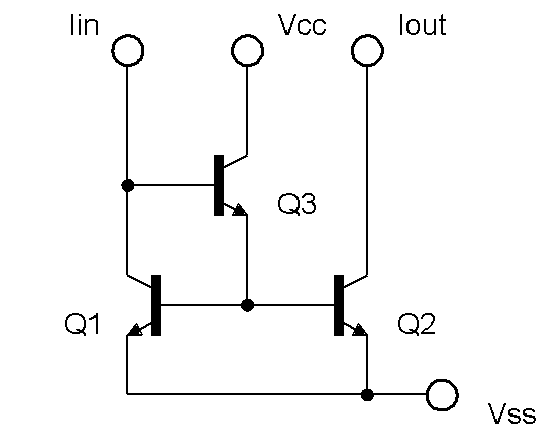
\includegraphics[scale=0.5]{obrazky/ZlepseneWilsonovoZrcadloNPN}
  \end{center}
  \caption{Zlepšené Wilsonovo proudové zrcadlo.}
\end{figure}

%% Konec dokumentu
\end{document}
